\documentclass[11pt,letterpaper]{article}
\usepackage[margin=0.83in,headheight=15pt]{geometry}
\usepackage[T1]{fontenc}
\usepackage{lmodern,microtype}
\usepackage[table]{xcolor}
\usepackage{graphicx,booktabs,tabularx,longtable,array,ragged2e}
\usepackage{enumitem,amsmath,amssymb}
\usepackage{tikz}
\usetikzlibrary{arrows.meta,positioning,fit,calc,shapes.geometric}
\usepackage{listings,fancyhdr,titlesec,caption,tocloft}
\setlength{\cftbeforesecskip}{1pt}
\usepackage[hidelinks]{hyperref}
\definecolor{navy}{HTML}{17324D}
\definecolor{teal}{HTML}{007E87}
\definecolor{muted}{HTML}{506579}
\definecolor{pale}{HTML}{EFF5F7}
\definecolor{linegray}{HTML}{CDD9E0}
\definecolor{ink}{HTML}{202C36}
\hypersetup{colorlinks=true,linkcolor=navy,urlcolor=teal,citecolor=teal,pdftitle={Software Repository Comprehension and Architecture Reverse Engineering: A Systematic Engineering Methodology},pdfsubject={Architecture reconstruction, static and dynamic analysis, security engineering}}
\color{ink}
\setlength{\parindent}{0pt}
\setlength{\parskip}{5pt}
\setlist{nosep,leftmargin=1.45em,topsep=3pt}
\setcounter{tocdepth}{2}
\titleformat{\section}{\Large\bfseries\color{navy}}{\thesection}{0.7em}{}[\vspace{2pt}\color{linegray}\titlerule]
\titleformat{\subsection}{\large\bfseries\color{teal}}{\thesubsection}{0.65em}{}
\titlespacing*{\section}{0pt}{14pt}{8pt}
\titlespacing*{\subsection}{0pt}{10pt}{4pt}
\pagestyle{fancy}\fancyhf{}
\fancyhead[L]{\small\color{muted} REPOSITORY COMPREHENSION}
\fancyhead[R]{\small\color{muted} TECHNICAL GUIDE / 1.0}
\fancyfoot[L]{\footnotesize\color{muted} Software architecture reverse engineering}
\fancyfoot[R]{\small\thepage}
\renewcommand{\headrulewidth}{0.4pt}
\renewcommand{\footrulewidth}{0pt}
\newcolumntype{Y}{>{\RaggedRight\arraybackslash}X}
\newcolumntype{P}[1]{>{\RaggedRight\arraybackslash}p{#1}}
\newcommand{\code}[1]{\texttt{\detokenize{#1}}}
\newcommand{\gate}[1]{\par\noindent\colorbox{pale}{\parbox{\dimexpr\linewidth-2\fboxsep\relax}{\textbf{\color{teal}Exit gate.} #1}}\par}
\newcommand{\evidence}[1]{\textbf{Evidence:} #1}
\newcommand{\tablehead}[2]{\rowcolor{navy}\color{white}\textbf{#1}&\color{white}\textbf{#2}\\}
\newcommand{\checkitem}[1]{\(\square\)\hspace{0.4em}#1}
\lstset{basicstyle=\small\ttfamily,breaklines=true,columns=fullflexible,keepspaces=true,showstringspaces=false,frame=single,rulecolor=\color{linegray},backgroundcolor=\color{pale},keywordstyle=\color{teal}\bfseries,commentstyle=\color{muted},stringstyle=\color{navy},aboveskip=6pt,belowskip=6pt}
\captionsetup{hypcap=false,font=small,labelfont=bf,textfont=it}
\tikzset{unit/.style={draw=navy,rounded corners=3pt,fill=pale,align=center,minimum height=10mm,font=\small,inner sep=5pt},external/.style={unit,fill=white,draw=muted},flow/.style={-{Latex[length=2mm]},thick,draw=teal},boundary/.style={draw=muted,dashed,rounded corners,inner sep=9pt},lbl/.style={font=\scriptsize,fill=white,inner sep=2pt,text=ink}}
\begin{document}
\hypersetup{pageanchor=false}% unnumbered cover
\begin{titlepage}
\thispagestyle{empty}
\noindent{\color{teal}\rule{\linewidth}{4pt}}\par
\vspace{0.55in}
{\large\bfseries\color{teal} SOFTWARE ENGINEERING / TECHNICAL METHODOLOGY\par}
\vspace{0.35in}
{\fontsize{33}{39}\selectfont\bfseries\color{navy} Software Repository\\Comprehension and\\Architecture Reverse\\Engineering\par}
\vspace{0.24in}
{\LARGE\color{muted} A Systematic Engineering Methodology\par}
\vspace{0.45in}
{\large A field guide to evidence-driven codebase analysis, architecture reconstruction, runtime verification, application security, and sustainable documentation.\par}
\vfill
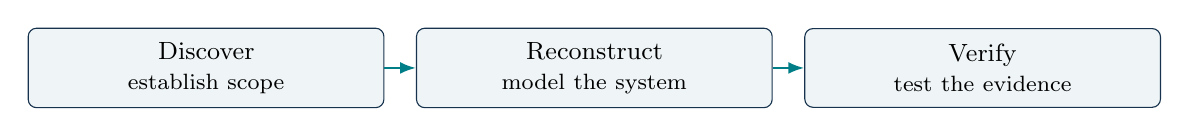
\begin{tikzpicture}[node distance=4mm]
\node[unit,text width=1.64in] (a) {Discover\\\footnotesize establish scope};
\node[unit,right=of a,text width=1.64in] (b) {Reconstruct\\\footnotesize model the system};
\node[unit,right=of b,text width=1.64in] (c) {Verify\\\footnotesize test the evidence};
\draw[flow] (a)--(b);\draw[flow] (b)--(c);
\end{tikzpicture}
\vfill

\noindent\begin{tabularx}{\linewidth}{@{}P{1.35in}Y@{}}
\textbf{Version} & 1.0 --- November 2026\\
\textbf{Audience} & Software engineers, architects, AppSec engineers, SREs, technical leads, and repository-analysis agents\\
\textbf{Scope} & Language-neutral methodology with Python examples; not a certification or audit of a specific repository\\
\end{tabularx}
\vspace{0.2in}
\noindent{\color{teal}\rule{\linewidth}{1pt}}
\end{titlepage}\hypersetup{pageanchor=true}
\pagenumbering{roman}
\section*{Executive summary}
Repository comprehension is the disciplined construction of a working mental model of a software system from its source code, configuration, tests, documentation, operational behavior, and change history. Architecture reverse engineering transforms these observations into higher-level abstractions that explain responsibilities, dependencies, execution paths, and security boundaries. The objective is not to read every file; it is to answer stakeholder questions with reproducible evidence and sufficient confidence to make safe engineering decisions.

This guide defines seven iterative phases: repository discovery, architecture analysis, static code analysis, dynamic analysis, security analysis, knowledge validation, and architecture documentation. Each phase specifies tasks, evidence, outputs, and acceptance criteria. The approach combines top-down discovery with bottom-up reconstruction and prioritizes one end-to-end workflow before expanding coverage.

The methodology draws on architecture reconstruction research from the Software Engineering Institute \cite{sei}, the C4 model \cite{c4}, architecture-description concepts associated with ISO/IEC/IEEE 42010:2022 \cite{iso}, and OWASP threat modeling \cite{owasp}. It is an original practical synthesis, not a normative interpretation or formal conformance assessment of the standard.

\subsection*{What success looks like}
A reviewer can identify the analyzed revision, explain how a representative request crosses components, locate the implementation and tests behind each architectural claim, distinguish verified facts from hypotheses, identify security-relevant trust transitions, and reproduce the verification procedure. Unresolved questions and inaccessible environments remain explicit.

\subsection*{How to use this guide}
For onboarding, emphasize discovery and the primary workflow. For a feature or defect, expand only the affected dependency neighborhood. For security assessment, extend the workflow into trust boundaries, alternate paths, authorization checks, and sensitive-data handling. For architecture documentation, maintain cross-view consistency and evidence traceability. The worked example is illustrative rather than a claim about an existing codebase.
\clearpage
\begingroup
\small
\setlength{\parskip}{0pt}
\tableofcontents
\endgroup
\clearpage
\pagenumbering{arabic}
\section{Foundations and operating principles}
\subsection{Terminology and scope}

\noindent\begin{tabularx}{\linewidth}{@{}P{1.7in}Y@{}}
\tablehead{Concept}{Working definition}
Repository comprehension & Understanding behavior, responsibilities, and constraints sufficiently to carry out a defined engineering task.\\
Architecture reconstruction & Recovering architectural abstractions from implementation artifacts and observations.\\
Static analysis & Inspecting source, syntax, dependencies, and configuration without executing the target program.\\
Dynamic analysis & Observing actual behavior under a specified execution environment and workload.\\
Architecture description (AD) & A structured expression of an architecture using views and related information.\\
Trust boundary & A transition across which identity, authority, confidentiality, or integrity assumptions change.\\
\bottomrule
\end{tabularx}
\subsection{Principles}
\begin{enumerate}
\item \textbf{Scope before depth.} Define the entity of interest, revision, target questions, permissions, and exclusions before exploring.
\item \textbf{Trace a vertical slice.} Follow one behavior from stimulus to outcome before exploring all modules horizontally.
\item \textbf{Separate intent from implementation.} Documentation describes intended behavior; source and configuration describe candidate behavior; runtime evidence describes behavior in a tested context.
\item \textbf{Reconstruct, do not invent.} Infer abstractions only when justified by artifacts and explicitly mark missing evidence.
\item \textbf{Verify proportionally.} Critical claims require stronger verification than low-impact descriptive details.
\item \textbf{Preserve operational safety.} Never run unfamiliar code against production systems or expose credentials during analysis.
\item \textbf{Maintain traceability.} Store claims, sources, revision, confidence, and validation status together.
\end{enumerate}
\subsection{Analysis contract}
Before work starts, record the repository URL, commit SHA, branch or tag, analysis date, environment, stakeholders, objectives, timebox, permitted actions, and expected deliverables. For multi-repository systems, record the revision of each dependency and identify what is outside the analysis boundary. Changes to the scope require an explicit record.
\gate{A reviewer can identify the target revision, purpose, authorized actions, and success conditions without relying on verbal context.}
\clearpage
\section{Methodology and evidence model}
\begin{center}
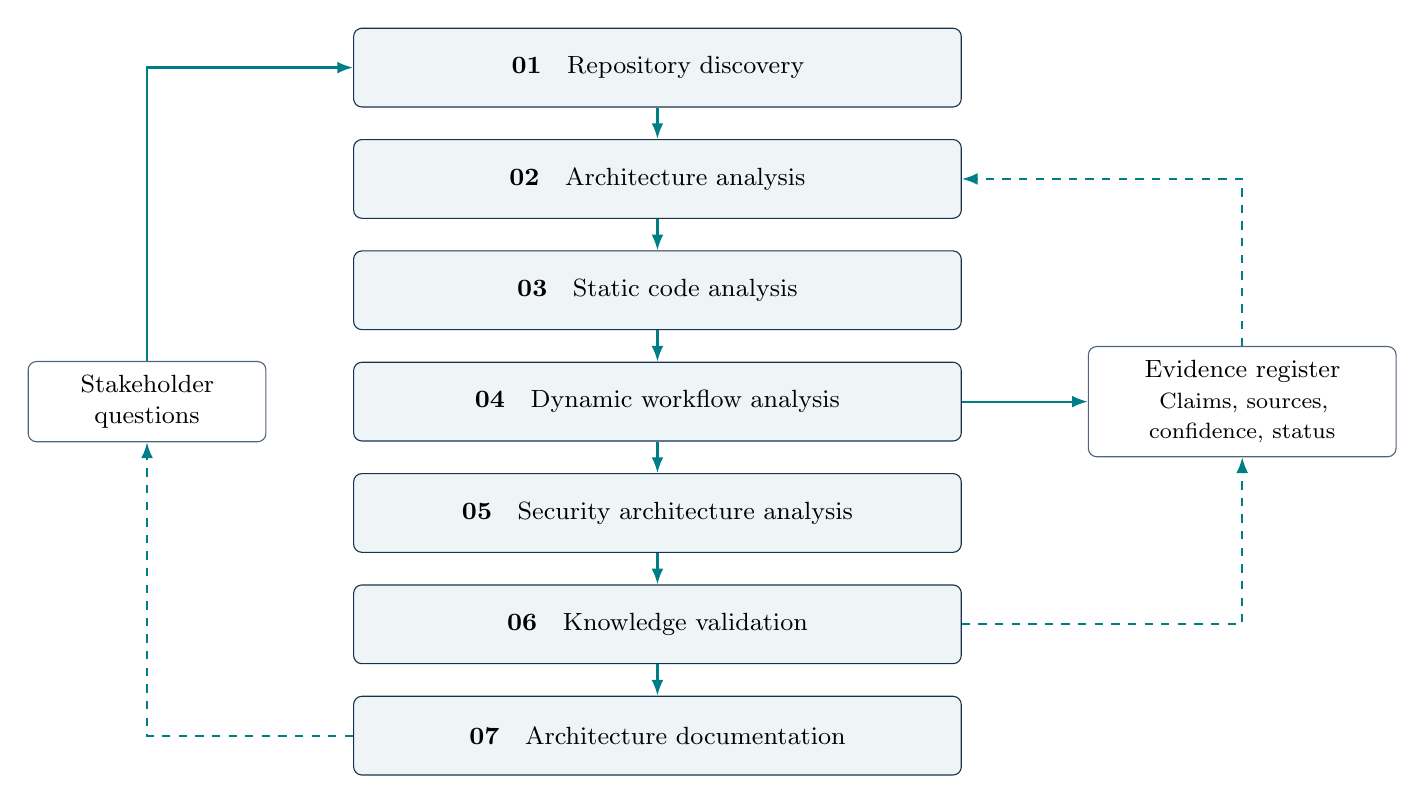
\begin{tikzpicture}[node distance=4mm]
\foreach \i/\labeltext in {1/Repository discovery,2/Architecture analysis,3/Static code analysis,4/Dynamic workflow analysis,5/Security architecture analysis,6/Knowledge validation,7/Architecture documentation}{
\ifnum\i=1 \node[unit,text width=2.9in] (p\i) {\textbf{0\i}\quad \labeltext};
\else \pgfmathtruncatemacro{\prev}{\i-1}\node[unit,below=of p\prev,text width=2.9in] (p\i) {\textbf{0\i}\quad \labeltext};\draw[flow] (p\prev)--(p\i);\fi}
\node[external,right=16mm of p4,text width=1.4in] (e) {Evidence register\\\footnotesize Claims, sources, confidence, status};
\draw[flow] (p4)--(e);\draw[flow,dashed] (e.north) |- (p2.east);\draw[flow,dashed] (p6.east) -| (e.south);
\node[external,left=11mm of p4,text width=1.05in] (q) {Stakeholder\\questions};
\draw[flow] (q.north) |- (p1.west);\draw[flow,dashed] (p7.west) -| (q.south);
\end{tikzpicture}
\captionof{figure}{Iterative reconstruction workflow. Solid arrows show the primary progression; dashed arrows show feedback and re-analysis.}
\end{center}
\subsection{Evidence classification}

\noindent\begin{tabularx}{\linewidth}{@{}P{1.45in}Y@{}}
\tablehead{Status}{Meaning and handling}
Observed & Directly supported by a specific file, configuration, test result, or trace. Cite the artifact and context.\\
Inferred & Reasoned from one or more observations. State assumptions and propose a verification step.\\
Contradicted & Evidence sources disagree. Record both, investigate, and avoid publishing a definitive claim.\\
Unknown & Insufficient or inaccessible evidence. Record the blocker and impact on the analysis.\\
\bottomrule
\end{tabularx}
Confidence is separate from status: high means strong, relevant evidence (preferably independent corroboration); medium means plausible but limited evidence; low means material uncertainty. An observed statement is not automatically a verified system-wide invariant. Keep a claim ID, artifact location, revision, environment, observation, inference, confidence, validation result, and reviewer. Do not copy secrets or sensitive payloads into evidence.
\clearpage
\section{Phase 1 --- Repository discovery}
\textbf{Objective.} Establish what the software does, how it is organized, and what is required to build, test, and operate it. Start read-only.
\subsection{Inventory the repository}

\noindent\begin{tabularx}{\linewidth}{@{}P{2.05in}Y@{}}
\tablehead{Artifact or location}{Questions to answer}
\code{README.md}, \code{docs/} & What problem does the project solve? What are its public capabilities and known constraints?\\
\code{CONTRIBUTING.md}, \code{AGENTS.md} & What development conventions and agent-specific instructions apply? Are instructions trustworthy and authorized?\\
\code{pyproject.toml},\newline \code{package.json}, \code{go.mod} & What language, runtime, dependencies, entry points, and scripts are declared?\\
Lockfiles, build manifests & What versions are resolved? Are dependencies pinned or reproducible?\\
Dockerfiles, Compose, IaC & What execution environments, services, ports, identities, and resource assumptions exist?\\
\code{.github/workflows/}, CI config & How are builds, tests, scans, packaging, and deployment performed?\\
\code{.env.example}, config files & What settings, feature flags, endpoints, and credentials are expected? Never print live secrets.\\
\code{tests/}, fixtures & What behaviors and boundary conditions are encoded as expectations?\\
License, ownership, history & Who owns components? What licenses, change patterns, and support constraints apply?\\
\bottomrule
\end{tabularx}
\subsection{Read-only orientation commands}
\begin{lstlisting}[language=bash]
git rev-parse HEAD
git status --short
git ls-files
git log --oneline -20
git shortlog -sn HEAD
tree -L 3 -a -I '.git|node_modules|.venv|dist'
rg --files --hidden -g '!.git' -g '!node_modules'
\end{lstlisting}
The commands assume a local Git checkout and installed tools. Use targeted searches rather than dumping sensitive configuration. Check ignored files, submodules, generated code, and monorepo workspaces only when relevant. Do not interpret a directory name as proof of architectural style.
\subsection{Outputs and safety gate}
Record a repository inventory, technology matrix (declared versus observed versions), build and test entry points, external dependency register, ownership map, and initial questions. Inspect install scripts, Git hooks, build plugins, CI actions, dependency lifecycle scripts, container mounts, privileges, and network access before any execution.
\gate{Inventory identifies major source, test, configuration, build, and deployment locations or marks them absent/unknown. Execution is not authorized by discovery alone.}
\clearpage
\section{Phase 2 --- Architecture analysis}
\textbf{Objective.} Recover system boundaries, major responsibilities, connectors, deployment assumptions, and architectural constraints. Combine top-down documentation with bottom-up evidence from imports, interface implementations, composition roots, configuration, and deployment manifests.
\subsection{Identify architectural patterns by evidence}

\noindent\begin{tabularx}{\linewidth}{@{}P{1.55in}Y@{}}
\tablehead{Candidate pattern}{Evidence to look for}
Layered architecture & Directional dependencies among presentation, business logic, and persistence.\\
Hexagonal architecture & Core-defined ports, external adapters, and dependency direction toward the application/domain core.\\
Modular monolith & Single deployable with meaningful internal module boundaries and explicit interfaces.\\
Microservices & Independently deployable services with explicit remote contracts; directories alone are insufficient.\\
Event-driven & Producers, consumers, event schemas, broker/topic configuration, and delivery semantics.\\
Agent-based & Model interaction, tool registry, runtime control loop, state, policy enforcement, and external tool execution.\\
\bottomrule
\end{tabularx}
\subsection{Use C4 at the appropriate depth}
The C4 model uses four static levels and supplementary diagrams \cite{c4}. Choose diagrams that answer stakeholder questions; not every repository needs all levels.

\noindent\begin{tabularx}{\linewidth}{@{}P{1.35in}Y@{}}
\tablehead{Diagram}{Scope and questions}
System context & Who uses the system? Which external systems does it interact with?\\
Container & What applications and data stores comprise the system? How do they communicate? A C4 container is not necessarily a Docker container.\\
Component & What major responsibilities and interfaces exist within one container?\\
Code & Which selected classes, functions, interfaces, or modules realize a component?\\
Dynamic / deployment & How do elements interact for a use case? Where do software instances run?\\
\bottomrule
\end{tabularx}
\subsection{Reconstruction procedure}
Identify external actors and systems; enumerate runnable applications and data stores; locate each application's composition root; cluster code by responsibility; map explicit dependencies; verify cross-boundary calls; compare declared and observed deployment topology; and record contradictions. Maintain consistent element identifiers across views. A package import is not proof of a network connection, and an IaC resource declaration is not proof of a live deployment.
\gate{Context and container views are supported by cited artifacts. Critical component boundaries and dependencies are identified; inferred or unknown topology is labeled.}
\clearpage
\subsection{Illustrative architecture views}
The following example is a hypothetical order-query API. Its diagrams are explanatory models, not findings from a real repository. Arrows show directional interaction; dashed outlines denote scope, not automatically a security boundary.
\begin{center}
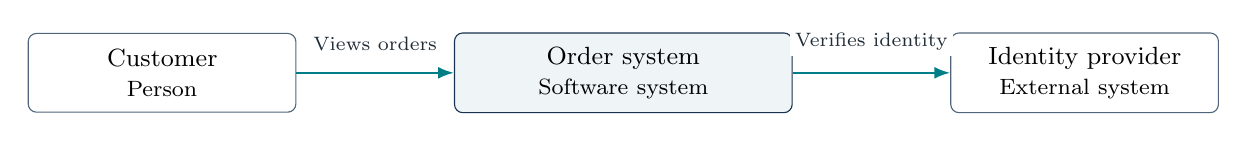
\begin{tikzpicture}[node distance=20mm]
\node[external,text width=1.2in] (user) {Customer\\\footnotesize Person};
\node[unit,right=of user,text width=1.55in] (sys) {Order system\\\footnotesize Software system};
\node[external,right=of sys,text width=1.2in] (idp) {Identity provider\\\footnotesize External system};
\draw[flow] (user)--node[lbl,above,yshift=2mm]{Views orders}(sys);\draw[flow] (sys)--node[lbl,above,yshift=2mm]{Verifies identity}(idp);
\end{tikzpicture}
\captionof{figure}{C4 system context --- order-query system.}
\vspace{12pt}
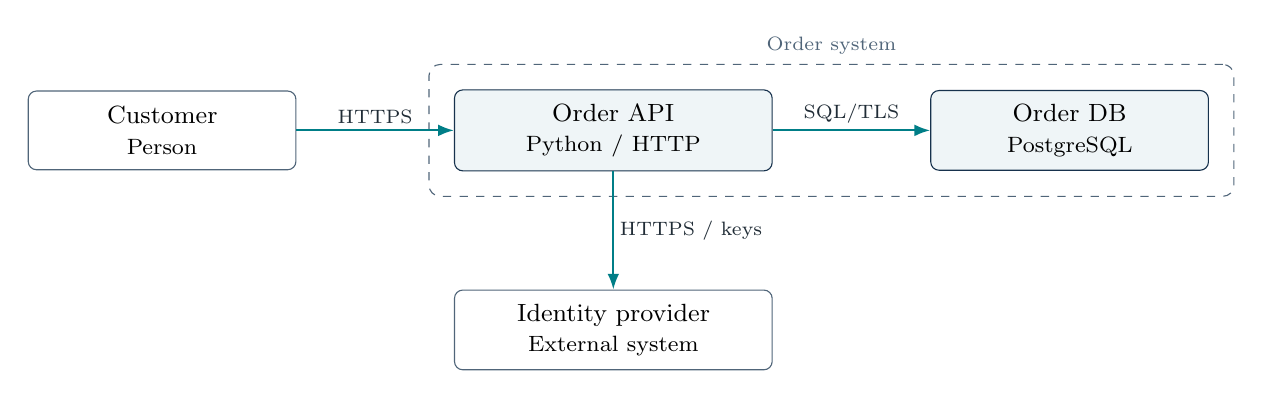
\begin{tikzpicture}[node distance=20mm]
\node[external,text width=1.2in] (user) {Customer\\\footnotesize Person};
\node[unit,right=of user,text width=1.45in] (api) {Order API\\\footnotesize Python / HTTP};
\node[unit,right=of api,text width=1.25in] (db) {Order DB\\\footnotesize PostgreSQL};
\node[external,below=15mm of api,text width=1.45in] (idp) {Identity provider\\\footnotesize External system};
\node[boundary,fit=(api)(db),label={[font=\scriptsize,text=muted]above:Order system}] {};
\draw[flow] (user)--node[lbl,above]{HTTPS}(api);\draw[flow] (api)--node[lbl,above]{SQL/TLS}(db);\draw[flow] (api)--node[lbl,right]{HTTPS / keys}(idp);
\end{tikzpicture}
\captionof{figure}{C4 container view --- API and data store.}
\vspace{12pt}
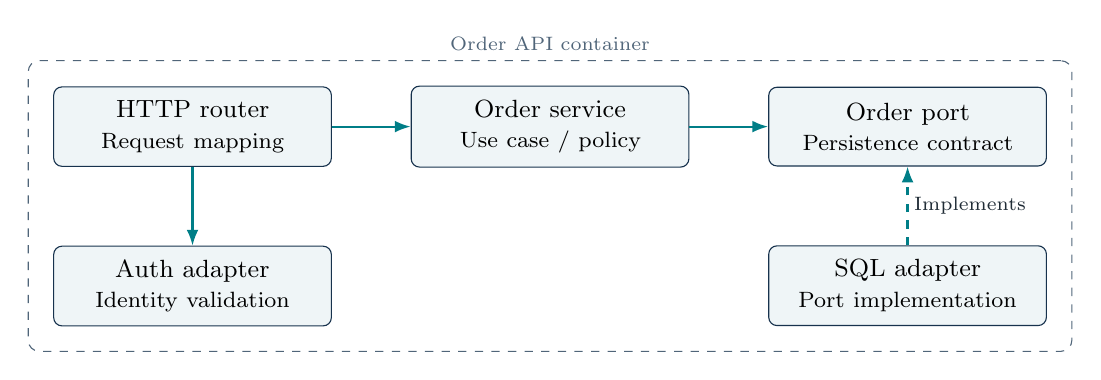
\begin{tikzpicture}[node distance=10mm]
\node[unit,text width=1.25in] (route) {HTTP router\\\footnotesize Request mapping};
\node[unit,right=of route,text width=1.25in] (svc) {Order service\\\footnotesize Use case / policy};
\node[unit,right=of svc,text width=1.25in] (port) {Order port\\\footnotesize Persistence contract};
\node[unit,below=of port,text width=1.25in] (adapter) {SQL adapter\\\footnotesize Port implementation};
\node[unit,below=of route,text width=1.25in] (auth) {Auth adapter\\\footnotesize Identity validation};
\node[boundary,fit=(route)(svc)(port)(adapter)(auth),label={[font=\scriptsize,text=muted]above:Order API container}]{};
\draw[flow] (route)--(svc);\draw[flow] (svc)--(port);\draw[flow] (route)--(auth);\draw[flow,dashed] (adapter)--node[lbl,right]{Implements}(port);
\end{tikzpicture}
\captionof{figure}{C4 component view --- arrows represent uses; dashed arrow indicates implementation of a contract.}
\end{center}
\textbf{Diagram review:} include title, scope, legend, element type and responsibility, labeled relationships, relevant technology, and links to evidence. Use a UML class diagram only where code-level relationships add explanatory value.
\clearpage
\section{Phase 3 --- Static code analysis}
\textbf{Objective.} Establish possible execution paths, data transformations, module coupling, and implementation contracts without running the target software.
\subsection{Locate execution entry points}
Inspect process entry points, package scripts, CLI registrations, HTTP routes, message consumers, scheduled jobs, serverless handlers, plugin hooks, and dependency-injection bindings. Trace definitions and references rather than relying solely on text matching. IDE semantic navigation and GitHub code navigation can help locate definitions and uses \cite{githubnav}.
\begin{lstlisting}[language=bash]
# Examples for a Python service; adapt to the framework.
rg -n 'if __name__|def main\(' --glob '*.py'
rg -n '@(app|router)\.(get|post|put|delete)' src
rg -n 'class .*Repository|def get_order' src tests
rg -n 'Depends\(|Protocol|ABC' src
# Replace example paths with paths found during discovery.
git log --follow -- src/orders/service.py
git blame -L 20,60 -- src/orders/service.py
\end{lstlisting}
\subsection{Analysis techniques}

\noindent\begin{tabularx}{\linewidth}{@{}P{1.55in}Y@{}}
\tablehead{Technique}{Purpose and caveats}
Call graph & Identify candidate caller/callee relationships; reflection and dispatch can hide edges.\\
Control-flow graph & Model branches, loops, returns, and exception paths. A syntactic path may be infeasible.\\
Data-flow analysis & Track value propagation across assignments, calls, serialization, and persistence.\\
Taint analysis & Track influence from untrusted sources to sensitive sinks, accounting for sanitizers and validators. CodeQL provides data-flow modeling facilities \cite{codeql}.\\
Dependency analysis & Examine imports, package references, interfaces, cycles, fan-in and fan-out. Distinguish source, build, and runtime dependencies.\\
Test analysis & Identify behavior contracts, assertions, mocks, edge cases, and untested assumptions. Passing tests cover only their exercised cases.\\
History analysis & Inspect changes, decisions, ownership and co-change patterns; correlation is not causation.\\
\bottomrule
\end{tabularx}
\subsection{Produce a static trace}
For each step, record the symbol, file and line range, incoming data, outgoing call, dependency binding, conditional branch, and relevant test. Follow the request until it reaches its terminal outcome, including errors. Note unresolved dispatch and framework-generated behavior for runtime verification.
\gate{At least one primary workflow has a source-linked trace from entry point to outcome, with important alternate branches and unresolved edges identified.}
\clearpage
\section{Phase 4 --- Dynamic analysis and workflow tracing}
\textbf{Objective.} Confirm what actually happens in a controlled environment and reconcile runtime behavior with static predictions.
\subsection{Prepare a safe execution environment}
Use an isolated disposable VM or restricted container with a nonprivileged identity, no host secrets or production endpoints, minimal network egress, and resource limits. Review build steps before execution; pin dependencies where practical, use synthetic fixtures, and record environment variables by name only. Isolation is a mitigation, not a guarantee. Where safe setup cannot be established, mark dynamic validation blocked.
\subsection{Run and observe a representative use case}
\begin{enumerate}
\item Establish baseline build and test status, including skipped and failed tests.
\item Select a deterministic scenario and expected outcome, with fixture and configuration IDs.
\item Capture a correlation identifier, entry point, major calls, state changes, and exit status.
\item Exercise an alternate or error path and verify cleanup, rollback, and error translation.
\item Compare trace with source analysis; record differences and repeat with controlled changes.
\end{enumerate}
\begin{center}
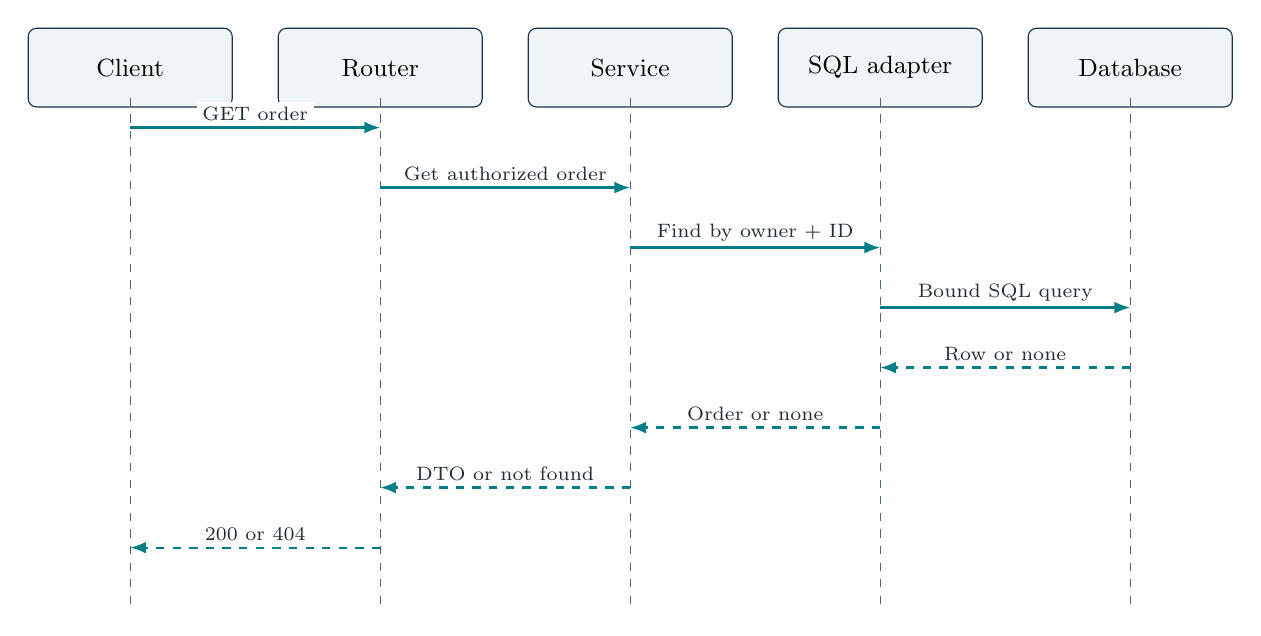
\begin{tikzpicture}[x=1.25in,y=0.30in]
\foreach \i/\n in {0/Client,1/Router,2/Service,3/SQL adapter,4/Database}{\node[unit,minimum width=1.02in] at (\i,0) {\n};\draw[muted,dashed] (\i,-0.5)--(\i,-9);}
\foreach \a/\b/\y/\t in {0/1/1/GET order,1/2/2/Get authorized order,2/3/3/Find by owner + ID,3/4/4/Bound SQL query}{\draw[flow] (\a,-\y)--node[lbl,above]{\t}(\b,-\y);}
\foreach \a/\b/\y/\t in {4/3/5/Row or none,3/2/6/Order or none,2/1/7/DTO or not found,1/0/8/200 or 404}{\draw[flow,dashed] (\a,-\y)--node[lbl,above]{\t}(\b,-\y);}
\end{tikzpicture}
\captionof{figure}{Illustrative sequence: authorized order lookup. Solid arrows are calls; dashed arrows are returns. Identity validation occurs at the router before this slice.}
\end{center}
\subsection{Runtime evidence}
Collect sanitized logs, debugger observations, traces, coverage, request/response metadata, and test results. Record versions, commands, timestamps and correlation IDs. A trace proves an observed path only under its recorded conditions; it does not establish that other paths are impossible.
\gate{One happy path and one meaningful failure/denial path are executed and reconciled, or a documented blocker explains why runtime evidence could not be collected.}
\clearpage
\section{Phase 5 --- Security architecture analysis}
\textbf{Objective.} Determine where untrusted data, authority, and sensitive state enter, move through, and leave the software. Apply threat modeling to the actual implementation, not only intended design \cite{owasp}.
\subsection{Map assets, boundaries, and controls}
\begin{center}
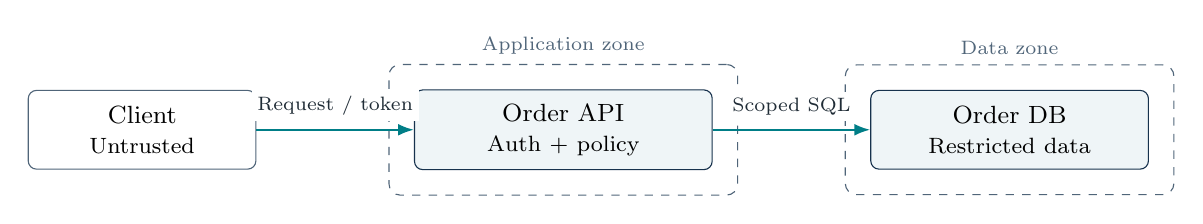
\begin{tikzpicture}[node distance=20mm]
\node[external,text width=1.0in] (client) {Client\\\footnotesize Untrusted};
\node[unit,right=of client,text width=1.35in] (api) {Order API\\\footnotesize Auth + policy};
\node[unit,right=of api,text width=1.25in] (db) {Order DB\\\footnotesize Restricted data};
\node[boundary,fit=(api),label={[font=\scriptsize,text=muted]above:Application zone}]{};
\node[boundary,fit=(db),label={[font=\scriptsize,text=muted]above:Data zone}]{};
\draw[flow] (client)--node[lbl,above,yshift=1mm]{Request / token}(api);\draw[flow] (api)--node[lbl,above,yshift=1mm]{Scoped SQL}(db);
\end{tikzpicture}
\captionof{figure}{Simplified security data-flow view. Dashed outlines designate trust zones; arrows show selected forward data flows. Return data and external identity flows should be modeled in a full assessment.}
\end{center}

\noindent\begin{tabularx}{\linewidth}{@{}P{1.45in}Y@{}}
\tablehead{Security concern}{Verification questions}
Attack surface & Which routes, listeners, jobs, webhooks, parsers, plugins, and privileged operations accept input?\\
Identity and authority & Who authenticates the caller? Where is resource-level authorization enforced? Is tenant scope preserved?\\
Input and output & Are schemas, canonicalization, encoding, file paths, queries, and outbound destinations constrained?\\
Sensitive data & What is collected, stored, logged, transmitted, retained, and deleted? Are secrets excluded from evidence?\\
Isolation and failure & What identities, filesystem/network permissions, limits and fail-closed behaviors apply?\\
Supply chain & Which dependencies, build scripts, CI permissions, provenance, and artifact controls are present?\\
Auditability & Which security-relevant decisions are recorded, correlated, and protected against tampering?\\
\bottomrule
\end{tabularx}
\subsection{Threat modeling with STRIDE}
For each asset, flow, and trust boundary, consider spoofing, tampering, repudiation, information disclosure, denial of service, and elevation of privilege. Describe a threat scenario, preconditions, potential impact, existing controls, verification evidence, residual risk, owner, and recommended treatment. Prioritize by exploitability and business impact; a scanner result is a candidate finding until investigated. Test only with authorization and non-production data.
\gate{Critical assets, entry points, trust boundaries, and control locations are mapped. High-impact threats have a validation plan or explicit limitation.}
\clearpage
\subsection{Application security verification and agent harnesses}

\noindent\begin{tabularx}{\linewidth}{@{}P{1.35in}Y@{}}
\tablehead{Method}{Use and limitations}
SAST & Identify insecure code patterns and potentially dangerous flows. Review reachability and framework semantics.\\
SCA & Identify vulnerable or unsupported dependencies. Validate version resolution, exposure, and applicability.\\
Secret scanning & Detect suspected credentials without reproducing values. Use approved validation and rotation procedures; avoid unauthorized live credential tests.\\
IaC scanning & Inspect intended infrastructure, IAM, and network configuration; validate live state separately when authorized.\\
DAST & Exercise a permitted test deployment; coverage depends on authentication, routes, and scanner configuration.\\
Manual review & Assess business logic, authorization, trust assumptions, and cross-component behavior missed by tools.\\
\bottomrule
\end{tabularx}
\textbf{AI-assisted repository analysis.} An agent harness adds a new security boundary between model proposals and execution authority. Repository content, tool outputs, issue text, and fetched documentation can contain adversarial instructions. Treat them as evidence, not as authority to grant permissions.
\begin{center}
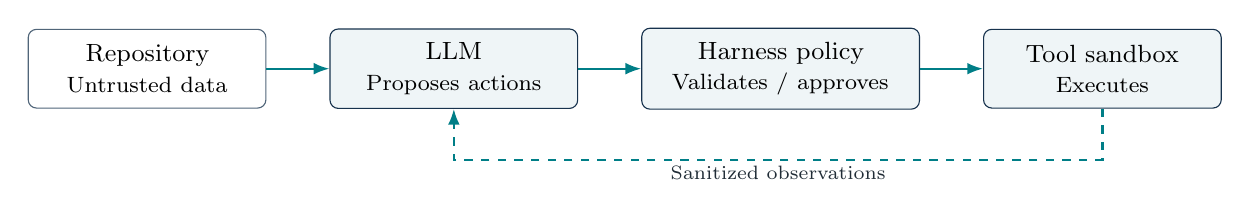
\begin{tikzpicture}[node distance=8mm]
\node[external,text width=1.05in] (repo) {Repository\\\footnotesize Untrusted data};
\node[unit,right=of repo,text width=1.10in] (model) {LLM\\\footnotesize Proposes actions};
\node[unit,right=of model,text width=1.25in] (policy) {Harness policy\\\footnotesize Validates / approves};
\node[unit,right=of policy,text width=1.05in] (tool) {Tool sandbox\\\footnotesize Executes};
\draw[flow] (repo)--(model);\draw[flow] (model)--(policy);\draw[flow] (policy)--(tool);
\draw[flow,dashed] (tool.south) -- ++(0,-0.65) -| node[pos=.25,lbl,below]{Sanitized observations} (model.south);
\end{tikzpicture}
\captionof{figure}{Agent-assisted analysis: the model proposes, the harness authorizes, the sandbox executes. The feedback path carries untrusted observations.}
\end{center}
Enforce scoped read-only tools by default, validated arguments, bounded execution, isolated storage, least-privilege credentials, and explicit approval for writes, network access, or sensitive operations. Preserve an audit trail and verify AI-generated descriptions against source evidence. Do not upload private repository material to unapproved services.
\subsection{Finding template}
\textbf{ID / title:} SEC-001 --- example resource-authorization gap (hypothetical). \textbf{Evidence:} commit, source location, reproducible test. \textbf{Impact:} cross-tenant disclosure if confirmed. \textbf{Status:} candidate / confirmed / rejected. \textbf{Treatment:} enforce owner scope in the service and persistence query; verify with a negative test. \textbf{Owner / residual risk:} assigned during review. Avoid rating a hypothetical issue as a verified vulnerability.
\clearpage
\section{Phase 6 --- Knowledge validation}
\textbf{Objective.} Demonstrate that the reconstructed model predicts behavior and supports safe changes. Validation should falsify assumptions, not merely confirm them.
\subsection{Build a verification matrix}

\noindent\begin{tabularx}{\linewidth}{@{}P{1.7in}Y Y@{}}
\rowcolor{navy}\color{white}\textbf{Claim}&\color{white}\textbf{Method}&\color{white}\textbf{Acceptance evidence}\\
Entry point dispatches use case & Trace source and run a representative test & Expected handler and service invocation observed.\\
Ownership limits access & Negative integration test using separate synthetic identities & No unauthorized data returned; policy outcome recorded.\\
Persistence is replaceable & Substitute a test adapter at the composition root & Service tests pass without real database access.\\
Failure handling is bounded & Inject approved dependency failure & Expected error, timeout or rollback; no sensitive output.\\
Diagram matches implementation & Review claims and compare to source/trace & Each critical node and edge has evidence or an explicit qualifier.\\
\bottomrule
\end{tabularx}
\subsection{Controlled modification}
Create a disposable branch or isolated copy. Choose a low-risk change: add a unit test, improve a log message without sensitive content, or fix a small deterministic bug. Define expected impact before editing. Run targeted tests, then relevant regression checks. Compare the result to the predicted dependency and execution paths. Revert or retain the change only as authorized. Never alter the baseline solely to make a test pass.
\begin{lstlisting}[language=bash]
# After approval, in an isolated disposable checkout:
git switch -c analysis/verify-order-flow
python -m pytest tests/test_order_service.py -q
python -m pytest -q
# Optional, if pytest-cov is installed:
python -m pytest --cov=src --cov-report=term-missing
# Review proposed changes before committing or publishing.
git diff --stat
git diff --check
\end{lstlisting}
\subsection{Measure evidence coverage, not just test coverage}
Define denominators before measurement. If $C$ is the set of in-scope critical architecture claims and $V$ is the subset with accepted verification evidence, report $|V|/|C|$ as a percentage only when $|C|>0$. Also report workflow coverage and unresolved high-impact questions with their counts and scope. Test line coverage is an auxiliary measure, not proof of architecture or security correctness.
\gate{Baseline and verification results are preserved. Critical claims have accepted evidence or named exceptions. A controlled change is validated where authorized; otherwise the omission is recorded.}
\clearpage
\section{Phase 7 --- Architecture documentation}
\textbf{Objective.} Transform discoveries into a maintainable architecture description that supports stakeholder decisions. ISO/IEC/IEEE 42010:2022 addresses architecture descriptions for diverse entities \cite{iso}; this guide uses a practical subset of its concepts and does not assert clause-level compliance.
\subsection{Stakeholders, concerns, and viewpoints}

\noindent\begin{tabularx}{\linewidth}{@{}P{1.25in}Y Y@{}}
\rowcolor{navy}\color{white}\textbf{Stakeholder}&\color{white}\textbf{Concern}&\color{white}\textbf{Proposed view}\\
Developer & Change impact, contracts, dependencies & Component, code, dynamic\\
Architect & Boundaries, coupling, decisions & Context, container, dependency\\
AppSec engineer & Trust, authority, data exposure & Data flow, threat and control\\
SRE / operator & Deployment, failure, observability & Deployment, dynamic, operations\\
Product owner & Capabilities and external interactions & Context and use-case summary\\
\bottomrule
\end{tabularx}
A viewpoint defines conventions for constructing a view that addresses concerns. For each selected viewpoint, document the purpose, audience, notation, modeling conventions, and review rules. A view applies those conventions to the entity under analysis. Maintain correspondences across views (for example, the same API container appears in its deployment and component views). Record inconsistencies and the evidence supporting decisions. Avoid presenting reconstructed rationale as an original historical design decision without an ADR or other evidence.
\subsection{Architecture description package}
\begin{lstlisting}
docs/
  repository-analysis/   # scope, inventory, dependency map
  architecture/
    architecture-description.md
    stakeholders-and-concerns.md
    viewpoints.md
    decisions-and-assumptions.md
    diagrams/            # context, container, component,
                         # selected code, sequence, deployment
  security/              # threats, assets, controls, findings
  verification/          # baseline, tests, traces, review
  evidence/              # claim register, source references
\end{lstlisting}
\subsection{Maintain the description}
Keep diagram sources and the claim register version-controlled. Associate each release or review with a revision. Update affected views when interfaces, dependencies, deployment topology, authorization, or data classification changes. Review diagrams for consistency and accessibility; keep sanitized evidence under appropriate access controls.
\gate{Architecture description includes scope, concerns, views, evidence, known gaps, decisions or assumptions, and review status. Diagrams are reproducibly rendered and reviewed.}
\clearpage
\section{Worked example: Python order-query service}
This synthetic example demonstrates the methodology without assuming a particular real repository. Paths, code and expected results below are illustrative; no application runtime has been executed for this guide.
\begin{lstlisting}
order-api/
  pyproject.toml
  src/orders/
    api.py                # HTTP adapter and identity binding
    service.py            # Application use case
    ports.py              # Persistence interface
    sql_adapter.py        # SQL implementation
    bootstrap.py          # Dependency composition
  tests/
    test_order_service.py
    test_order_api.py
  Dockerfile
  compose.yaml
\end{lstlisting}
\subsection{Source-level model}
\begin{lstlisting}[language=Python]
# ports.py (illustrative)
from dataclasses import dataclass
from typing import Protocol

@dataclass(frozen=True)
class Order:
    id: str
    owner_id: str

class OrderRepository(Protocol):
    def find_owned(self, order_id: str,
                   owner_id: str) -> Order | None: ...

# service.py (illustrative; imports shown)
from .ports import Order, OrderRepository

class OrderService:
    def __init__(self, repo: OrderRepository):
        self.repo = repo

    def get_order(self, order_id: str,
                  principal_id: str) -> Order | None:
        order = self.repo.find_owned(order_id, principal_id)
        if order is None or order.owner_id != principal_id:
            return None
        return order
\end{lstlisting}
The core service depends on a persistence contract rather than a concrete database driver. The HTTP adapter must obtain the principal from a validated identity, not a caller-supplied owner ID. The SQL adapter should bind parameters and scope the query by both order ID and owner ID. A no-match result can be translated to a uniform 404 to reduce resource-existence disclosure; this does not replace authentication or monitoring.
\clearpage
\subsection{Trace the primary and alternate paths}

\noindent\begin{tabularx}{\linewidth}{@{}P{1.45in}Y Y@{}}
\rowcolor{navy}\color{white}\textbf{Step}&\color{white}\textbf{Expected behavior}&\color{white}\textbf{Evidence to collect}\\
HTTP request & GET order with validated identity & Route definition, auth middleware, integration trace\\
Use case & Invoke service with order ID and principal & Service call site and unit test\\
Port invocation & Delegate owner-scoped lookup & Interface and composition root\\
Persistence & Bind values in a scoped SELECT & SQL adapter, query test, sanitized trace\\
Result & Return allowed order or no match & Service result, response schema\\
Failure & Deny other owner's order; handle DB error & Negative integration and failure injection tests\\
\bottomrule
\end{tabularx}
\subsection{Example negative unit test}
\begin{lstlisting}[language=Python]
from orders.ports import Order
from orders.service import OrderService

class BadAdapter:
    def find_owned(self, order_id, owner_id):
        # Simulate an adapter that returns another owner's row.
        return Order(order_id, "other-owner")

def test_service_rejects_foreign_order():
    service = OrderService(BadAdapter())
    assert service.get_order("order-1", "caller") is None
\end{lstlisting}
This test checks defense in depth at the service boundary. It does not establish that the HTTP adapter authenticates correctly or that the SQL adapter actually applies ownership scope. Add integration tests for valid identity, invalid identity, authorized access, cross-owner access, missing data, database failure, and parameter binding. Inspect logs to ensure no token or sensitive order content is captured.
\subsection{Example evidence record}

\noindent\begin{tabularx}{\linewidth}{@{}P{1.45in}Y@{}}
\tablehead{Field}{Example value (synthetic)}
Claim ID & ARCH-003: order service depends on a persistence port.\\
Source & \code{src/orders/service.py}, symbol \code{OrderService.__init__}; actual commit and lines to be captured in a real review.\\
Status / confidence & Observed in the illustrative listing; no real repository confidence assigned.\\
Verification & Proposed: inspect bootstrap binding; substitute fake adapter; run unit test.\\
Limitations & No checkout, runtime, database, or identity provider has been examined.\\
\bottomrule
\end{tabularx}
\clearpage
\section{Tooling and navigation playbook}
Tools are optional and language-dependent. Select tools for evidence quality, not for maximum output volume. Verify tool versions, permissions, and licensing before use.

\noindent\begin{tabularx}{\linewidth}{@{}P{1.35in}P{1.9in}Y@{}}
\rowcolor{navy}\color{white}\textbf{Category}&\color{white}\textbf{Example tools}&\color{white}\textbf{Primary output}\\
Discovery & Git, tree, ripgrep & Revision, inventory, textual matches\\
Semantic navigation & IDE LSP, Universal Ctags, Tree-sitter & Definitions, references, indexed syntax\\
Dependency analysis & pydeps, language build tools & Import and package relationships\\
Static security & Semgrep, CodeQL & Candidate findings and data-flow paths\\
Code modeling & Pyreverse, Doxygen, PlantUML & Class or dependency representations\\
Debugging & pdb, GDB, IDE debugger & Breakpoints, variables, stack traces\\
Tracing & OpenTelemetry, Jaeger & Correlated spans and timing\\
System observation & strace, tcpdump, Wireshark & System calls or network evidence (authorized only)\\
Testing & pytest, pytest-cov & Assertions, failures, coverage\\
Architecture documentation & PlantUML, C4-PlantUML, TikZ & Version-controlled diagram sources\\
\bottomrule
\end{tabularx}
\subsection{Diagram-as-code example}
The guide's figures use native TikZ for a self-contained LaTeX build. The following portable PlantUML example is a UML sequence diagram, not a C4 diagram. For C4 diagrams, use an appropriate C4 notation/library and pin its version locally rather than downloading unreviewed includes during CI.
\begin{lstlisting}
@startuml
 title Order lookup - authorized request
 actor Client
 participant Router
 participant OrderService as Service
 participant SqlAdapter as Adapter
 database PostgreSQL as DB
 Client -> Router: GET /orders/{id}
 Router -> Service: get_order(id, principal)
 Service -> Adapter: find_owned(id, principal)
 Adapter -> DB: parameterized SELECT
 DB --> Adapter: row or none
 Adapter --> Service: order or none
 Service --> Router: allowed order or none
 Router --> Client: 200 or 404
@enduml
\end{lstlisting}
\clearpage
\section{Timeboxed study and maturity levels}
The following ten-hour plan provides an initial orientation, not a guarantee of complete coverage. Expand the scope based on risk, complexity, accessibility, and stakeholder needs.

\noindent\begin{tabularx}{\linewidth}{@{}P{2.1in}P{0.75in}Y@{}}
\rowcolor{navy}\color{white}\textbf{Activity}&\color{white}\textbf{Time}&\color{white}\textbf{Output}\\
Discovery & 30 min & Scope and artifact inventory\\
Architecture discovery & 60 min & Context and container sketches\\
Static analysis & 90 min & Primary source-linked path\\
Runtime tracing & 90 min & Happy-path and error observations\\
Test analysis & 60 min & Behavioral contracts and coverage gaps\\
Security assessment & 90 min & Threats, trust boundaries, controls\\
Architecture documentation & 120 min & Views and evidence register\\
Implementation / validation & 60 min & Controlled test or modification\\
\midrule
\textbf{Total} & \textbf{600 min} & Initial ten-hour study\\
\bottomrule
\end{tabularx}
\subsection{Progressive depth}

\noindent\begin{tabularx}{\linewidth}{@{}P{1.4in}Y@{}}
\tablehead{Level}{Completion characteristics}
L1 --- Oriented & Can locate build, entry points, tests and major modules; understands purpose and scope.\\
L2 --- Mapped & Can explain context, container boundaries and one source-linked workflow; assumptions recorded.\\
L3 --- Verified & Runtime behavior and meaningful error paths are reconciled; critical claims have evidence.\\
L4 --- Assessed & In-scope threats, controls, failure modes, and material security risks are examined.\\
L5 --- Maintained & Architecture documentation is reviewed, versioned, traceable and updated through change governance.\\
\bottomrule
\end{tabularx}
These levels are an internal assessment rubric, not an industry standard. Assign the highest level whose required conditions are satisfied in the defined scope; do not silently waive blocked activities. Report static-only assessment separately if runtime execution is not permitted.
\subsection{Tailor the method to the task}
For onboarding, prioritize the smallest useful workflow and basic tests. For bug fixing, reconstruct the failing path before broad architecture work. For feature delivery, inspect upstream/downstream contracts and change impact. For security work, prioritize externally reachable and privileged paths. For legacy migration, extend analysis to deployment, persistence, external interfaces, and historical constraints.
\clearpage
\appendix
\section{Repository review checklist}
Record Pass, Fail, Not Applicable (with rationale), or Blocked (with owner and next action). A blocked item does not count as a pass. Apply the checklist to the agreed scope and evidence revision.
\begin{longtable}{@{}P{0.48in}P{3.0in}P{2.75in}@{}}
\rowcolor{navy}\color{white}\textbf{ID}&\color{white}\textbf{Acceptance criterion}&\color{white}\textbf{Expected evidence}\\\endhead
D01 & \checkitem{Revision and analysis scope recorded.} & Commit SHA, date, objectives, exclusions.\\
D02 & \checkitem{Major artifacts inventoried.} & Source, build, tests, config, CI, deployment or absence.\\
D03 & \checkitem{Execution safety assessed.} & Sandbox, script review, network and credential constraints.\\
A01 & \checkitem{System boundary and actors identified.} & Context view and external interfaces.\\
A02 & \checkitem{Applications and stores mapped.} & Container view, artifact links, assumptions.\\
A03 & \checkitem{Critical components and interfaces identified.} & Component inventory, composition root, dependency evidence.\\
S01 & \checkitem{Primary entry point located.} & File, symbol and route/handler binding.\\
S02 & \checkitem{Workflow statically traced.} & Source-linked steps, conditions, sinks and outcomes.\\
S03 & \checkitem{Key alternate paths mapped.} & Error, denial or timeout branch evidence.\\
R01 & \checkitem{Baseline captured.} & Environment, commands and test outcomes.\\
R02 & \checkitem{Primary runtime path verified.} & Sanitized trace or repeatable observation.\\
R03 & \checkitem{Failure path verified.} & Negative test/trace and cleanup behavior.\\
SEC01 & \checkitem{Assets and trust boundaries mapped.} & Data-flow view and asset classifications.\\
SEC02 & \checkitem{Critical controls examined.} & Authentication, authorization, validation and isolation evidence.\\
SEC03 & \checkitem{Material threats triaged.} & Finding status, risk, mitigation and owner.\\
V01 & \checkitem{Claims have validation status.} & Evidence register, unresolved contradictions.\\
V02 & \checkitem{Controlled change tested, if authorized.} & Diff, targeted tests and regression results.\\
AD01 & \checkitem{Views address stakeholder concerns.} & Stakeholder/viewpoint mapping.\\
AD02 & \checkitem{Diagram elements and edges traceable.} & Consistent names, types, scope, legends and evidence.\\
AD03 & \checkitem{Review and maintenance assigned.} & Reviewer, revision, gaps, next review trigger.\\
\bottomrule
\end{longtable}
\clearpage
\section{Reusable analysis record templates}
\subsection{Analysis charter}
\begin{lstlisting}
Repository / revision:
Entity of interest / scope:
Stakeholders and questions:
Primary workflow and expected outcome:
Out-of-scope components:
Authorized actions / prohibited actions:
Environment and isolation requirements:
Deliverables / acceptance gates:
Timebox / owner / reviewer:
\end{lstlisting}
\subsection{Evidence register (YAML example)}
\begin{lstlisting}
claim_id: ARCH-001
claim: "<one falsifiable statement>"
revision: "<commit SHA>"
status: inferred  # observed | inferred | contradicted | unknown
confidence: medium
sources:
  - path: "<repository-relative path>"
    lines: "<start-end>"
    symbol: "<symbol>"
observation: "<what the artifact actually shows>"
inference: "<reasoning and assumptions, if applicable>"
verification:
  method: "<test, trace, review or other procedure>"
  result: pending  # pass | fail | pending | blocked
  environment: "<environment identifier>"
limitations: "<coverage or evidence gaps>"
owner: "<review owner>"
\end{lstlisting}
\subsection{Workflow and architecture review record}
\begin{lstlisting}
Workflow ID / name:
Stimulus / actor / preconditions:
Step | component | symbol | input | output | evidence ID
Alternate paths / trust transitions:
Expected versus observed result:
Architecture view IDs affected:
Open questions / contradictions / risk:
Review decision / owner / next action:
\end{lstlisting}
\clearpage
\section{References and further reading}
\renewcommand{\refname}{}
The sources below support the core methodology. Tool examples and the worked case are original illustrative material; the standard's public description, rather than its full normative text, was used to establish its scope.
\begingroup
\renewcommand{\section}[2]{}
\begin{thebibliography}{99}
\raggedright
\bibitem{sei} L. O'Brien, C. Stoermer, and C. Verhoef, \emph{Architecture Reconstruction Guidelines, Third Edition}, Carnegie Mellon University Software Engineering Institute, CMU/SEI-2002-TR-034, 2003. \url{https://www.sei.cmu.edu/library/architecture-reconstruction-guidelines-third-edition/}.
\bibitem{c4} Simon Brown, \emph{The C4 Model: Diagrams}. \url{https://c4model.com/diagrams}.
\bibitem{iso} ISO/IEC/IEEE 42010:2022, \emph{Software, systems and enterprise --- Architecture description}. International Organization for Standardization, 2022. \url{https://www.iso.org/standard/74393.html}.
\bibitem{owasp} OWASP Cheat Sheet Series, \emph{Threat Modeling Cheat Sheet}. \url{https://cheatsheetseries.owasp.org/cheatsheets/Threat_Modeling_Cheat_Sheet.html}.
\bibitem{githubnav} GitHub Docs, \emph{Navigating code on GitHub}. \url{https://docs.github.com/en/repositories/working-with-files/using-files/navigating-code-on-github}.
\bibitem{codeql} GitHub CodeQL documentation, \emph{About data flow analysis}. \url{https://codeql.github.com/docs/writing-codeql-queries/about-data-flow-analysis/}.
\end{thebibliography}
\endgroup
\vspace{8pt}
\textbf{Final principle.} The value of an architecture reconstruction is determined by how well its claims explain the system, how reliably those claims can be verified, and how effectively the resulting description supports engineering decisions. Treat comprehension as a maintained body of evidence, not a one-time reading exercise.
\end{document}
